%************************************************
\chapter{The main theorem}
%************************************************

Let us state and recall the main theorem we want to prove.

\begin{theorem*}
    A finitely generated right-angled Coxeter group \(W\) has a finite index subgroup \(W'\), such that \(W'\) is residually finite and rationally solvable (RFRS).
\end{theorem*}

The goal of this whole chapter is to explain Agol's proof of this theorem, using the preliminaries and tools we have developed.
We will break the proof down into smaller pieces and will discuss in each section a specific aspect of the proof.


% ***********************************************
\section{The RFRS property}
% ***********************************************

We should state clearly what we have to show.
This is essentially the construction of a finite index subgroup, that is RFRS.
But what does it mean for a group \(G\) to be RFRS?
We shall start by giving the definition of the RFRS condition to shed some light onto our goal.

\begin{definition}
    Let \(G\) be a group.
    Then, \(G\) satisfies the RFRS condition, if there is a sequence of subgroups \(G = G_0 > G_1 > \ldots\), satisfying the following conditions.
    \begin{enumerate}
        \item for each \(i\), \(G_i \triangleleft G\) is a normal subgroup of \(G\),
        \item for each \(i\), the index of \(G_i\) in \(G\), \([G : G_i]\) is finite,
        \item the intersection \(\bigcap_i G_i = \{1\}\) is the trivial group, meaning the sequence is cofinal, and
        \item for each \(i\), the group \((G_i)_r^{(1)} := \ker\{G_i \to \Q \otimes_\Z (G_i)_{\text{ab}}\}\) is a subgroup of \(G_{i+1}\).
    \end{enumerate}
\end{definition}

Observe that in practice, it suffices to show that conditions \(2\) to \(4\) hold. % as once they are satisfied we can simply pass to the Core of each \(G_i\) in \(G\) and this new sequence will.
To justify this, let \(G = G_0 > G_1 > \cdots\) be a cofinal sequence of finite index subgroups \(G_i < G\) with \((G_i)_r^{(1)} \leq G_{i+1}\).
Then, for each \(i\), we pass to the core of \(G_i\) in \(G\), which is defined by Core\((G_i) := \bigcap_{g \in G} g G_i g^{-1}\).
By construction, the core of a subgroup \(G_i\) is normal in \(G\) and furthermore, we claim: %the following.
\Claimm{If \(G_i\) has finite index in \(G\), its core will also have finite index in \(G\).}
\Claimmproof{
    Let \(G_i\) be a subgroup in \(G\) with \([G : G_i] < \infty\).
    Then, \(G\) acts (by left multiplication) on the left cosets of \(G_i\) in \(G\) and the kernel of this action consists of the elements \(h \in G\) with
    \[hgG_i = gG_i \iff g^{-1}hgG_i = G_i \iff g^{-1}hg \in G_i \iff h \in gG_ig^{-1} \quad \forall g \in G.\]
    We note that the kernel is exactly the core of \(G_i\).
    Moreover, the quotient \(\faktor{G}{\text{Core}(G_i)}\) embeds into the symmetric group Sym\((\faktor{G}{G_i})\), as the left action on the cosets permutes them.
    As the order of this symmetric group is \([G : G_i]!\), we see that if \(G_i\) has finite index in \(G\), the core has finite index as well.
}
Thus, to see that this new sequence satisfies the RFRS condition, it remains to check that the rational derived subgroup \((\text{Core}(G_i))_r^{(1)}\) is a subgroup of the group Core\((G_{i+1})\).

\noindent
Clearly, for \(g \in G\) we have the equality \(g(G_i)_r^{(1)}g^{-1} = (gG_ig^{-1})_r^{(1)}\), from which we obtain
\[(\text{Core}(G_i))_r^{(1)} \leq \bigcap_{g \in G} (gG_ig^{-1})_r^{(1)} = \bigcap_{g \in G} g(G_i)_r^{(1)}g^{-1} \leq \bigcap_{g \in G} gG_{i+1}g^{-1} = \text{Core}(G_{i+1}).\]
To summarize, by accepting to pass to the sequence of core subgroups in \(G\), we can drop the first condition on the sequence of subgroups in the RFRS condition.

\begin{remark}\label{rmk:tensoring}
    Note that an abelian group \(A\) has a natural structure as a \(\Z\)-module.
    Thus, the tensor product with the rationals is well-defined and tensoring \(A\) with \(\Q\) kills the torsion part of the abelian group \(A\).
    % Note that tensoring an abelian group \(A\) (as \(\Z\)-module) with the rationals, `kills' the torsion part of \(A\), whence \(\Q \otimes_\Z A \cong \faktor{A}{\text{Torsion}}\).
    Whence, we have that \(\Q \otimes_\Z A \cong \Q \otimes_\Z \faktor{A}{\text{Torsion}}\).
    To see this, take an elementary tensor \(r \otimes a\) in \(\Q \otimes_\Z A\) so that \(a\) is a torsion-element of order \(n\).
    Then we get the following equalities,
    \[r \otimes a  = r \cdot \frac{n}{n} \otimes a = r \cdot \frac{1}{n} \otimes n\cdot a = 0.\]
    In particular, for the abelianization \(G_{\text{ab}}\), the group \(\Q \otimes_\Z G_{\text{ab}}\) is isomorphic to \(\Q \otimes_\Z \faktor{G_{\text{ab}}}{\text{Torsion}}\).
    Moreover, the torsion-free abelianization embeds into \(\Q \otimes_\Z G_{\text{ab}}\) and the so called rational derived subgroup \((G)_r^{(1)}\) is the kernel of the homomorphism from \(G\) to its torsion-free abelianization tensored with the rationals.
\end{remark}


% ***********************************************
\section{Construction of the manifold cover}
% ***********************************************

Consider the abelianization \(W_{\text{ab}}\) of \(W\), which is isomorphic to \((\Z/2\Z)^{n}\).
Now, the abelianization yields a homomorphism \(\alpha : W \to W_{\text{ab}}\).
In the following we will focus on its kernel \(\ker\alpha\). %, we will turn our attention to in the following.
Note that by the first homomorphism theorem, \(\ker\alpha\) has finite index in \(W\), since
\[\abs{\faktor{W}{\ker\alpha}} = \abs{\faktor{\Z}{2\Z}}^{n} = 2^{n} < \infty.\]
Here we used the fact that \(W\) is finitely generated, whence \(n = \abs{I} = \abs{S} < \infty\).

\noindent
Furthermore, note that for each \(J \subset I\) with \(W_J\) finite, we have an isomorphism between \(W_J\) and \((\faktor{\Z}{2\Z})^{\abs{J}}\).
Thus, the restriction of \(\alpha\) to each such subgroup \(\alpha\vert_{W_J}\) is an injective homomorphism.
We now use that in the right-angled case, the isotropy subgroups of codimension-\(k\) faces are all of this form.
This can be seen, as the isotropy subgroup of a codimension-\(k\) face \(F\) is generated by the reflections in the \(k\) codimension-\(1\) faces, whose intersection forms \(F\).
As all these codimension-\(1\) faces meet at right-angles, the generators commute pairwise.
Therefore, all isotropy subgroups inject into the abelianization of \(W\).
This implies that the intersection of an isotropy subgroup with the kernel of \(\alpha\) is trivial and consequently no isotropy group is contained in the kernel \(\ker\alpha\).
Since finite subgroups are contained in isotropy subgroups, the kernel \(\ker\alpha\) acts freely on the Tits cone \(WC\) corresponding to \(W\).

In particular, by \Cref{thm:stabilizer} the action of \(W\) on the interior of its Tits cone \(int(WC)\) is properly discontinuous.
By \Cref{thm:convexity} the Tits cone is also a convex cone, implying that it has trivial fundamental group, whence is simply-connected.
Having all this information, we are able to apply \Cref{lem:covering} to obtain that the following map is a covering
\[int(WC) \;\longrightarrow\; \faktor{int(WC)}{\ker\alpha} \qquad x \mapsto \text{Orb}_{\ker\alpha}(x).\]
% Using the local homeomorphism property of a covering map and the fact that the Tits cone \(WC\) is a subspace of \(\R^n\), we conclude that the quotient \(\faktor{int(WC)}{\ker\alpha}\) is indeed a manifold.
We conclude the results of this section in the following proposition.

\begin{proposition}
    Let \(W\) be a right-angled Coxeter group with corresponding Tits cone \(WC\).
    Then, there is a finite index subgroup \(W' \leq W\), acting by covering action on the interior of the Tits cone, implying that the quotient \(\faktor{int(WC)}{W'}\;\) is a manifold.
    It is given by \(W' = \ker\{W \to W_{\text{ab}}\} = \ker\alpha\).
\end{proposition}


% ***********************************************
\section{Some orbifold theory}
% ***********************************************

In this section, we want to elaborate more on the natural orbifold structure of the fundamental chamber \(C\).
We start by giving a formal definition of an orbifold.
We break the definition down into smaller pieces, starting with local models, sometimes called (orbifold) charts.

\begin{definition}
    A \emph{local model} is a pair \((\widetilde{U}, \Gamma)\), where \(\widetilde{U} \subset \R^n\) is open and \(\Gamma\) is a finite subgroup of the group of diffeomorphisms of \(\widetilde{U}\), denoted \emph{diffeo}\((\widetilde{U})\), acting on \(\widetilde{U}\).
    By abusing notation, we will sometimes say that the quotient \(U = \faktor{\widetilde{U}}{\Gamma}\;\) is the local model.
\end{definition}

Now that we have defined the local structure of an orbifold, we want to translate between these local models.
This is being made precise by orbifold maps.

\begin{definition}
    An \emph{orbifold map} between local models \((\widetilde{U}_i, \Gamma_i), (\widetilde{U}_j, \Gamma_j)\) is a pair of maps \((\widetilde{\psi}, \varphi)\),
    consisting of a smooth map \(\widetilde{\psi} : \widetilde{U}_i \to \widetilde{U}_j\) and a homomorphism of groups \(\varphi : \Gamma_i \to \Gamma_j\).
    We enforce the map \(\widetilde{\psi}\) to be \(\varphi\)-equivariant, meaning that for all \(g \in \Gamma_i\) and all \(\widetilde{x} \in \widetilde{U}_i\), \(\widetilde{\psi}(g\widetilde{x}) = \varphi(g)\widetilde{\psi}(\widetilde{x})\) holds.
    Then \(\widetilde{\psi}\) induces a map \(\psi : \faktor{\widetilde{U}_i}{\Gamma_i} \to \faktor{\widetilde{U}_j}{\Gamma_j}\), between the local models.
    When all three of these maps are injective, we call \(\psi\) a local isomorphism.
\end{definition}

Now that we have these local definitions, we `glue' them together, to obtain an orbifold.
Before we do so, we recall some notions from topology.

\noindent
Suppose, we are given an open cover \(\{U_i\}\) of a topological space \(X\).
It is said to be \emph{locally finite}, if every \(x \in X\) admits a neighborhood \(N\) such that \(N \cap U_i\) is empty for all but finitely many of the indices \(i\).
The open cover \(\{U_i\}\) is a \emph{refinement} of an open cover \(\{V_j\}\) of \(X\), if for every \(V_j\) there is a \(U_i\) with \(U_i \subseteq V_j\).
Now, the topological space \(X\) is said to be \emph{paracompact}, if every open cover of \(X\) admits such a locally finite refinement.

\begin{definition}
    An \(n\)-dimensional \emph{(smooth) orbifold} \(Q\) is a pair \((X_Q, \mathcal{A})\).
    The space \(X_Q\) is a paracompact Hausdorff space, called the \emph{underlying space}.
    The set \(\mathcal{A}\) is called an \emph{orbifold atlas}, consisting of charts \((U_i, \phi_i)\), indexed by some set \(I\) and satisfying the following conditions:
    \begin{itemize}
        \item the \(U_i\) form an open cover of the underlying space \(X_Q\),\vspace*{-.7em}
        \item for each \(U_i\) there exists a local model \(\faktor{\widetilde{U}_i}{\Gamma_i}\) with a homeomorphism \(\phi_i : U_i \to \faktor{\widetilde{U}_i}{\Gamma_i}\) and
        \item charts have to be compatible, meaning that for \(U_i \subset U_j\) the inclusion is a local isomorphism.
    \end{itemize}
\end{definition}

To sketch the connection between manifolds and orbifolds, let us mention one more thing.

\begin{definition}
    The \emph{local group} \(loc(x)\) of some \(x\) in a local model \(\faktor{\widetilde{U}}{\Gamma}\;\) is the isotropy group of any \(\widetilde{x}\) living in \(\widetilde{U}\), getting projected onto \(x\).
    The \emph{singular locus} \(\Sigma (Q)\) of an orbifold \(Q\) consists of all points in the underlying space \(X_Q\) with non-trivial local group, i.e. \(\Sigma(Q) = \{x \in X_Q \;\vert\; loc(x) \neq \{1\}\}\).
\end{definition}

By this definition, we see that an orbifold with empty singular locus is just a manifold.
Furthermore, when thinking about an orbifold, we can just think about the underlying space and label each element in the singular locus by its local group.

\noindent
Many basic examples arise by taking the quotient relative to a properly discontinuous group action on \(\R^n\).
We want to mention at least some examples.

\begin{example}
    \begin{enumerate}
        \item Consider the flat plane \(\R^2\) with the action of a cyclic group \(\faktor{\Z}{n\Z}\) by rotation about the origin.
            The arising orbifold is a cone with singular point the origin and cone angle \(\frac{2\pi}{n}\).
        
        \item Consider the sphere \(S^2\) with the action of a cyclic group \(\faktor{\Z}{n\Z}\) by rotation about the north pole \(N\).
            The arising orbifold now is called a \emph{teardrop} with singular point, the north pole \(N\).
    \end{enumerate}

    \begin{figure}[ht!]
        \label{fig:orbifolds}
        \centering
        \subfloat[\centering The cone orbifold.]{{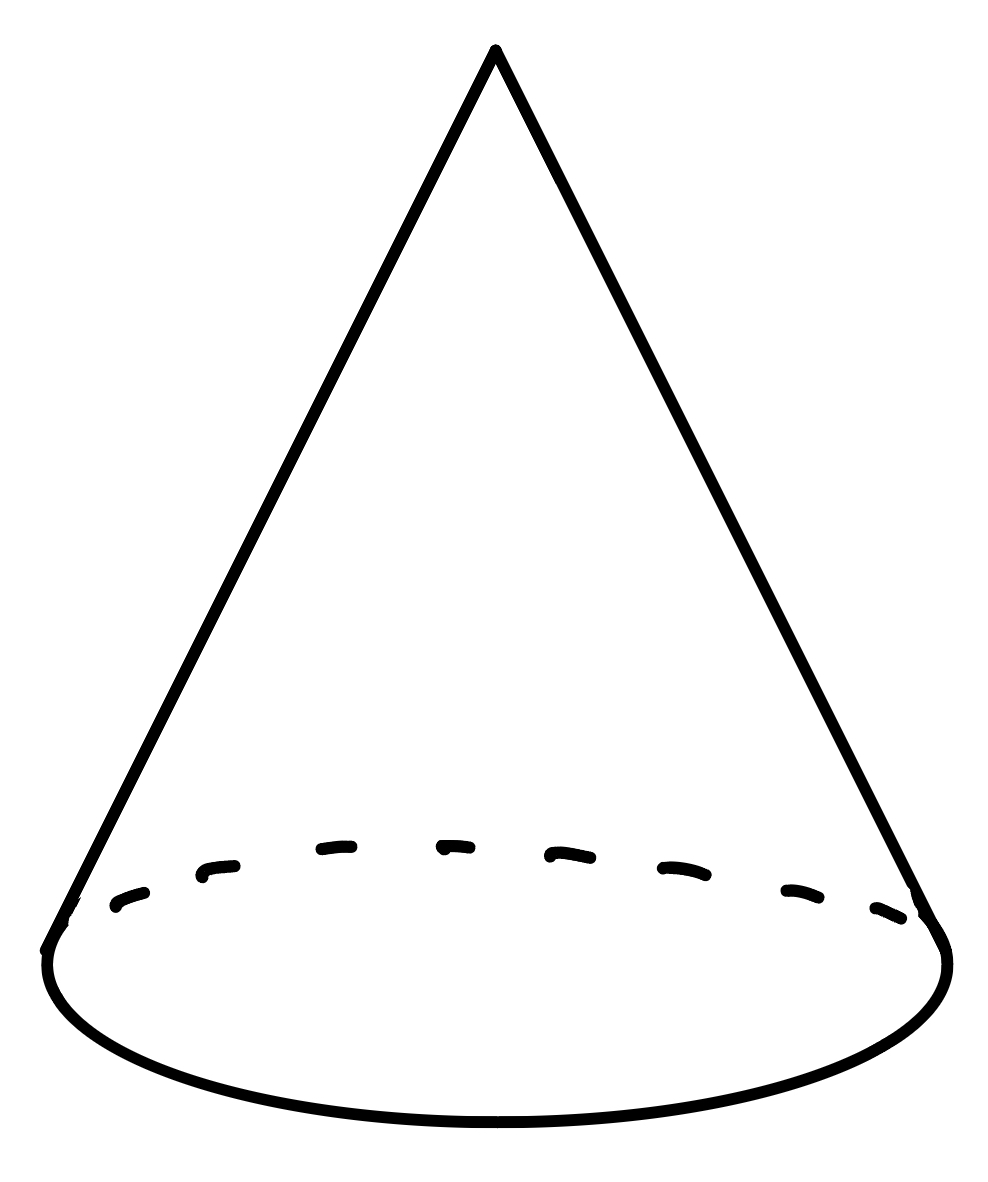
\includegraphics[height=4cm]{gfx/Cone.png}}}\hspace*{3cm}
        \subfloat[\centering The teardrop orbifold.]{{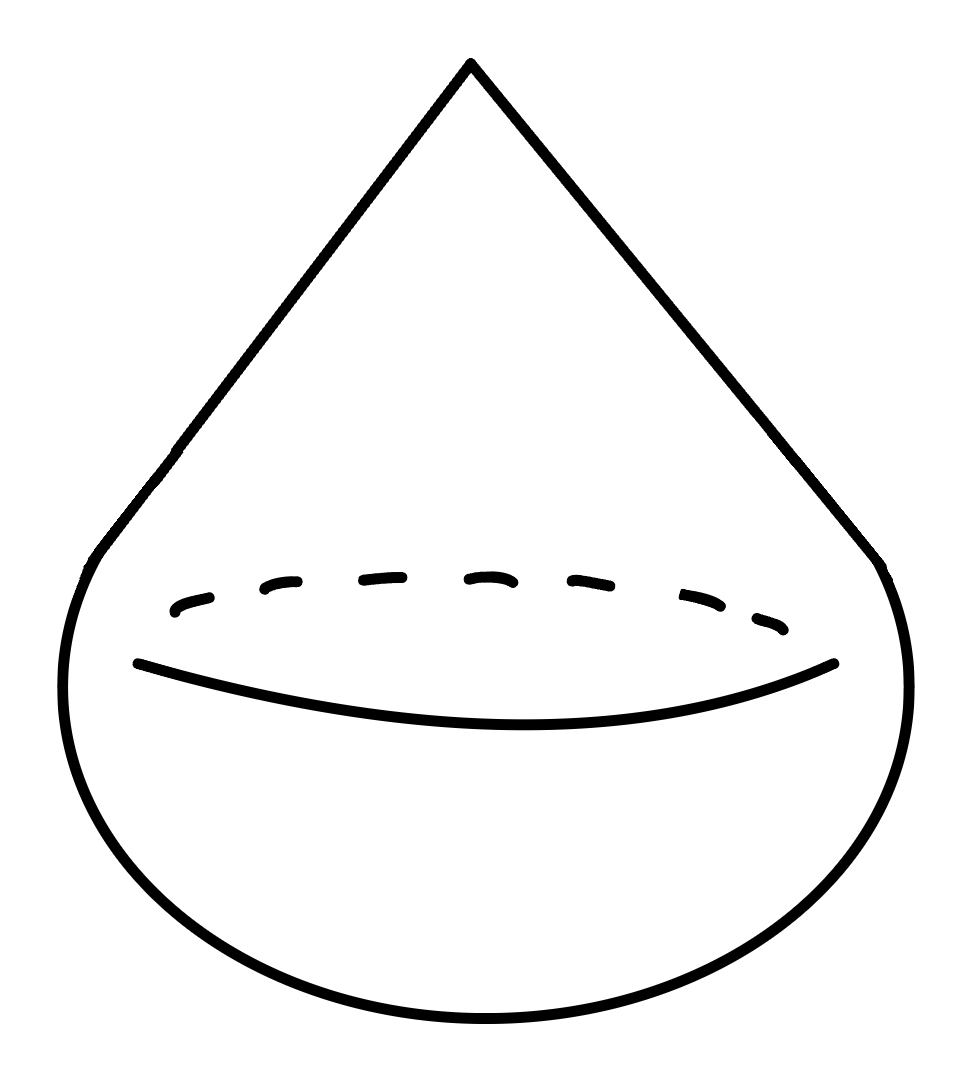
\includegraphics[height=4cm]{gfx/Teardrop.png}}}
    \end{figure}
\end{example}

% By starting with a topological space \(X\), this is actually a more general way to construct orbifolds.
% Given a properly discontinuously action of a group \(G\) on \(X\), simply pass to the quotient space \(\faktor{X}{G}\) to obtain an orbifold.
% In contrast, to obtain a manifold, one has to demand the action to be free as well.
% This is not the only analogy between manifolds and orbifolds.
The concept of orbifold coverings translates almost one to one from the ordinary case.

\begin{definition}
    An orbifold covering \(p: Q' \to Q\) is a continuous map on the underlying spaces \(X_{Q'} \to X_Q\), such that for each point \(x \in X_Q\) there is a local model \(U = \faktor{\widetilde{U}}{\Gamma}\) around \(x\) and each component \(V_i\) of \(p^{-1}(U)\) is homeomorphic to \(\faktor{\widetilde{U}}{\Gamma_i}\) for a subgroup \(\Gamma_i\) of \(\Gamma\).
    Furthermore, the restriction \(p\vert_{V_i} : V_i \to U\) corresponds to the natural projection \(\faktor{\widetilde{U}}{\Gamma_i} \to \faktor{\widetilde{U}}{\Gamma}\).
\end{definition}

\begin{remark}\label{rmk:covers}
    We want to mention here, that the universal cover of an orbifold is exactly what we think of, i.e. the initial object in the category of orbifold coverings.
    Moreover, there is a notion of orbifold fundamental groups, which we won't define here.
    For us it is only important to know that they behave to orbifold covers the same as fundamental groups to coverings in the ordinary case.
    In particular, subgroups (of index \(n\)) of the orbifold fundamental group correspond to (\(n\)-sheeted) orbifold coverings.
\end{remark}
    
Having all this in mind, we have two ways of approaching the fundamental chamber \(C\).
One way, it obtains its natural orbifold structure as the quotient \(\faktor{int(WC)}{W}\).
As the Tits cone is simply connected, it is the universal cover of \(C\) and we observe that the orbifold fundamental group of \(C\) is precisely \(W\).
On the other hand, the fundamental chamber is the quotient of the manifold \(\faktor{int(WC)}{W'}\) by a finite group action.
\vspace*{\parskip}

\begin{figure}[h!]
    \begin{minipage}[c]{.6\textwidth}
        Since \(W'\) is a finite index subgroup of \(W\), \Cref{rmk:covers} implies that we get a covering map \(p\) so that the diagram on the right commutes.
        Thus, both of the approaches to the fundamental chamber \(C\) agree in the sense that the projection map \(int(WC) \to \faktor{int(WC)}{W}\) factors through the manifold cover, constructed in Section \(3.1\).
    \end{minipage}\quad
    \begin{minipage}{.35\textwidth}\vspace*{-1em}
        \begin{tikzcd}
            int(WC) \arrow[r] \arrow[d] & \faktor{int(WC)}{W} \\
            \faktor{int(WC)}{W'} \arrow[ru, "p"', dashed]
        \end{tikzcd}
    \end{minipage}
\end{figure}


% ***********************************************
\section{The cofinal cover}
% ***********************************************

In this section, we \emph{sketch} the proof of the existence of a cofinal sequence of two-fold covers, arising by iteratively reflecting in faces.
Some more results from the theory of orbifolds would be needed for the whole proof.
Since they go beyond the scope of this work, we will state and use them without proof.

In the following, doubling along faces means the construction of a sequence of right-angled polytopes \(P_k = P_{k-1} \cup g_{k-1}(P_{k-1})\), where \(g_{k-1}\) is the reflection in one of the faces of the previous polytope \(P_{k-1}\), denoted by \(F_{k-1}\).
The following proposition will tell us, that in the case of a right-angled Coxeter group, we are able to double the fundamental chamber \(C\) in one of its faces and are still able to cover the whole Tits cone \(WC\) by reflecting in the faces of the resulting polytope.

\begin{proposition}\label{prop:double}
    Let \(P_k \subset \R^n\) be a right-angled polytope with orbifold structure, coming from a doubling sequence starting in \(P_0 = C\).
    Denote its orbifold fundamental group by \(\pi_1^{\text{orb}}(P_k)\) and its universal cover by \(\widetilde{P}\).
    Then, the fundamental group \(\pi_1^{\text{orb}}(P_{k+1})\) is isomorphic to the group generated by reflections in the faces of the double \(P_{k+1}\).
    Furthermore, the fundamental group \(\pi_1^{\text{orb}}(P_{k+1})\) of the double is an index-\(2\) subgroup of \(\pi_1^{\text{orb}}(P_k)\) and the following two conditions are satisfied.
    \begin{enumerate}
        \item \(\forall k \in \N: \forall g \in \pi_1^{\text{orb}}(P_k): g(\mathring{P}_k) \cap \mathring{P}_k \neq \emptyset \implies g = 1\), and
        \item \(\forall k \in \N: \bigcup_{g \in \pi_1^{\text{orb}}(P_k)} g(P_{k}) = \widetilde{P}\).
    \end{enumerate}
\end{proposition}
\begin{proof}
    We will omit this proof here, as it goes beyond the scope of this work.
\end{proof}

To state the other auxiliary lemma we will need, we first want to show that each chamber in the Tits cone can uniquely be labeled by elements of its corresponding group.

\begin{lemma}\label{lem:labels}
    Let \(W\) be a Coxeter group and \(WC\) its Tits cone.
    The chambers of the form \(w(C)\) in the Tits cone can be labeled uniquely by elements in \(W\).
\end{lemma}
\begin{proof}
    Let \(v(C), w(C)\) be chambers in \(WC\) for \(v, w \in W\), such that \(v \neq w\) and \(w(C) = v(C)\).\newline
    But then, by \Cref{thm:stabilizer} we have that
    \[w(\mathring{C}) \cap v(\mathring{C}) = w(\mathring{C} \cap w^{-1}v(\mathring{C})) \neq \emptyset \implies w^{-1}v = 1 \iff w = v.\]
    Thus, the chambers can be labeled in a unique way.
\end{proof}

\begin{remark}
    We remark that each of the right-angled polytopes \(P_k\) can be decomposed into a union of translates of the fundamental chamber \(C\).
    This means for each polytope \(P_k\) there is a \(n_k \in \N\) and elements \(w_{i,k} \in W\), so that \(P_k = \bigcup_{i=1}^{n_k} w_{i,k}(C)\).
\end{remark}

We proceed with another helpful result, whose proof relies on the aforementioned results.

\begin{lemma}
    Let \(C \subset \R^n\) be the fundamental chamber of a Coxeter group \(W\).
    The non-trivial labels \(w_{i,k} \neq 1_W\) of the chambers, defining the polytope \(P_k = \bigcup_{i=1}^{n_k} w_{i,k}(C)\), are \emph{not} contained in the reflection group, generated by reflecting in its faces.
\end{lemma}
\begin{proof}
    Note that by \Cref{lem:labels}, the chambers of the form \(w(C)\) are uniquely labeled by the elements \(w \in W\).
    Thus, let \(P_k := \bigcup_{i = 1}^{n_k} w_{i,k}(C)\) be as in the lemma and \(w_{i,k}\) one of its defining labels.
    Assume, \(w_{i,k} \neq 1_W\) is contained in the reflection group generated by reflecting in the faces of \(P_k\).
    But then we have that \(w_{i,k}(\mathring{P}_k) \cap \mathring{P}_k \neq \emptyset\), contradicting \Cref{prop:double}.
\end{proof}

Using this insight, we define a graph \(G\) with vertices \(V(G) := \{w(C) \;\vert\; w \in W\}\) and edges \(E(G) := W \times S\).
The endpoint map is given by \(\delta : W \times S \to 2^{V(G)},\; (w, s) \mapsto (w(C), ws(C))\).
Thus, two vertices \(w(C)\) and \(v(C)\) have an edge, if there is an \(s \in S\), such that \(ws = v\).
Then, clearly we have \(wsw^{-1}w(C) = ws(C) = v(C)\).
Note that the element \(wsw^{-1}\) is the only element, that flips the edge \(\{w(C), ws(C)\}\).
Thus, the map \(W \times S \to W, \; (w, s) \mapsto wsw^{-1}\) defines a labeling of the edges by elements in \(W\).
We will call the combinatorial graph of \(G\) (meaning that every double edge gets collapsed) the \emph{chamber graph} Cham\((W, S)\) of \(W\).

% \begin{example}
%     In the case of the free product of \Cref{ex:freeprod}, by transporting everything to the poincaré disc, we see the following picture.
% \end{example}

This graph is canonically isomorphic to the combinatorial Cayley graph of the group \(W\) and we thus see that the Cayley graph `embeds' into the Tits cone \(WC\).

\begin{theorem}\label{thm:cofinal}
    There exists a cofinal doubling sequence \(P_k\), coming from the fundamental chamber \(P_0 = C\).
    This means that we have \(WC = \bigcup_{n \in \N} P_n\).
\end{theorem}
\begin{proof}
    The proof is by induction on the word length \(\ell(w)\).
    For \(\ell(w) = 0\), the corresponding chamber is the fundamental chamber \(C\), which is covered by itself.
    \IH{The chambers with labels \(v\) of length \(\ell(v) = k\) are covered by a polytope \(P_k = \bigcup_{i=1}^{n_k} w_{i,k}(C)\) \newline\hspace*{2em} in the doubling sequence \(\{P_k\}_{k \in \N}\).}\par\noindent
    We need to show that the chambers \(w(C)\) with labels \(w \in W\) of length \(\ell(w) = k + 1\) can be covered by doubling \(P_k\) finitely many times in faces.
    First observe that there is a label \(v\), whose chamber \(v(C)\) is contained in \(P_k\) and that is connected to \(w\) by an edge in the Cayles graph.
    Since the Cayley graph sits inside the Tits cone and is isomorphic to the chamber graph, the chambers \(w(C)\) and \(v(C)\) have to be adjacent, sharing a face that is contained in a face of \(P_k\).
    Then, we can distinguish two cases.
    Either, \(w(C)\) is already contained in \(P_k\) and we are done, or we double \(P_k\) in the face shared by \(v(C)\) and \(w(C)\), so that \(w(C)\) is contained in \(P_{k+1}\).
    Since \(W\) is finitely generated, there are finitely many more labels \(w' \in W\) of length \(\ell(w') = k + 1\) and we repeat the above procedure for each of them.
    Thus, every chamber in the Tits cone can be covered by doubling finitely many times in faces of the fundamental chamber \(C\).
    % We need to show that chambers of the form \(w(C)\) with \(\ell(w) = k\) can be covered by reflecting in a face of the polytope \(P\).
    % Using the chamber graph Cham\((W, S)\), constructed above, we deduce that for each such \(w\), there is a \(v \in W\) of length \(\ell(v) = k - 1\), connected to \(w\) by an edge in Cham\((W, S)\). % , labeled by \(ws_iw^{-1}\) for an \(i \in I\).
    % This is due to the fact that the chamber graph is isomorphic to the Cayley graph of  \(W\) and the length function of \(W\) is induced by the Cayley graph.
    % But then, the chamber \(w(C)\) is adjacent to the chamber \(v(C)\) and the latter is contained in \(P\) by \textbf{(IH)}.
    % Thus, either \(w(C)\) itself is already contained in \(P\) or we reflect in the face shared by \(w(C)\) and \(v(C)\) to cover \(w(C)\) with the double \(P'\) of \(P\).
    % Now, continuing with the next element \(w\) of length \(k\), we eventually double \(P'\) and repeat this for all such \(w\).
    % This iterative doubling process is valid by \Cref{prop:double} and by induction every chamber \(g(C)\) for \(g \in W\) can be covered.
\end{proof}

% The conclusion of this section is that the doubling sequence starting in the fundamental chamber \(C\) of the right-angled Coxeter group \(W\) is a cofinal sequence of two-fold (orbifold) covers.
% Thus, we conclude that the doubling sequence starting in the fundamental chamber \(C\) is a cofinal sequence of two-fold covers.

\begin{remark}\label{rmk:groupseries}
    % Using \Cref{prop:double}, we see that the cofinality of this sequence translates to the group side.
    % More precisely, this sequence of two-fold covers induces a sequence of index-\(2\) subgroups via the fundamental groups of the covering spaces.
    Note that by \Cref{prop:double} the elements corresponding to labels of chambers inside a right-angled polytope \(P_k\) are not contained in \(\pi_1^{\text{orb}}(P_k)\) and \(\pi_1^{\text{orb}}(P_{k+1})\) is a subgroup in \(\pi_1^{\text{orb}}(P_k)\) of index two.
    By \Cref{thm:cofinal} we have a doubling sequence \(\{P_k\}_{k \in \N}\) with \(\bigcup_{n \in \N} P_n = WC\).
    As the fundamental group of \(WC\) is trivial (it is a convex cone), the intersection of the fundamental groups of the \(P_k\) is trivial as well.
    Thus, the cofinality of the doubling sequence translates to the group side.
\end{remark}

\begin{example}
    As an example, transporting the Tits cone of the free product from \Cref{ex:freeprod} to the poincaré disc, a portion of the chamber graph is depicted below.
    \begin{figure}[h!]
        \label{fig:chambergraphex}
        \centering
        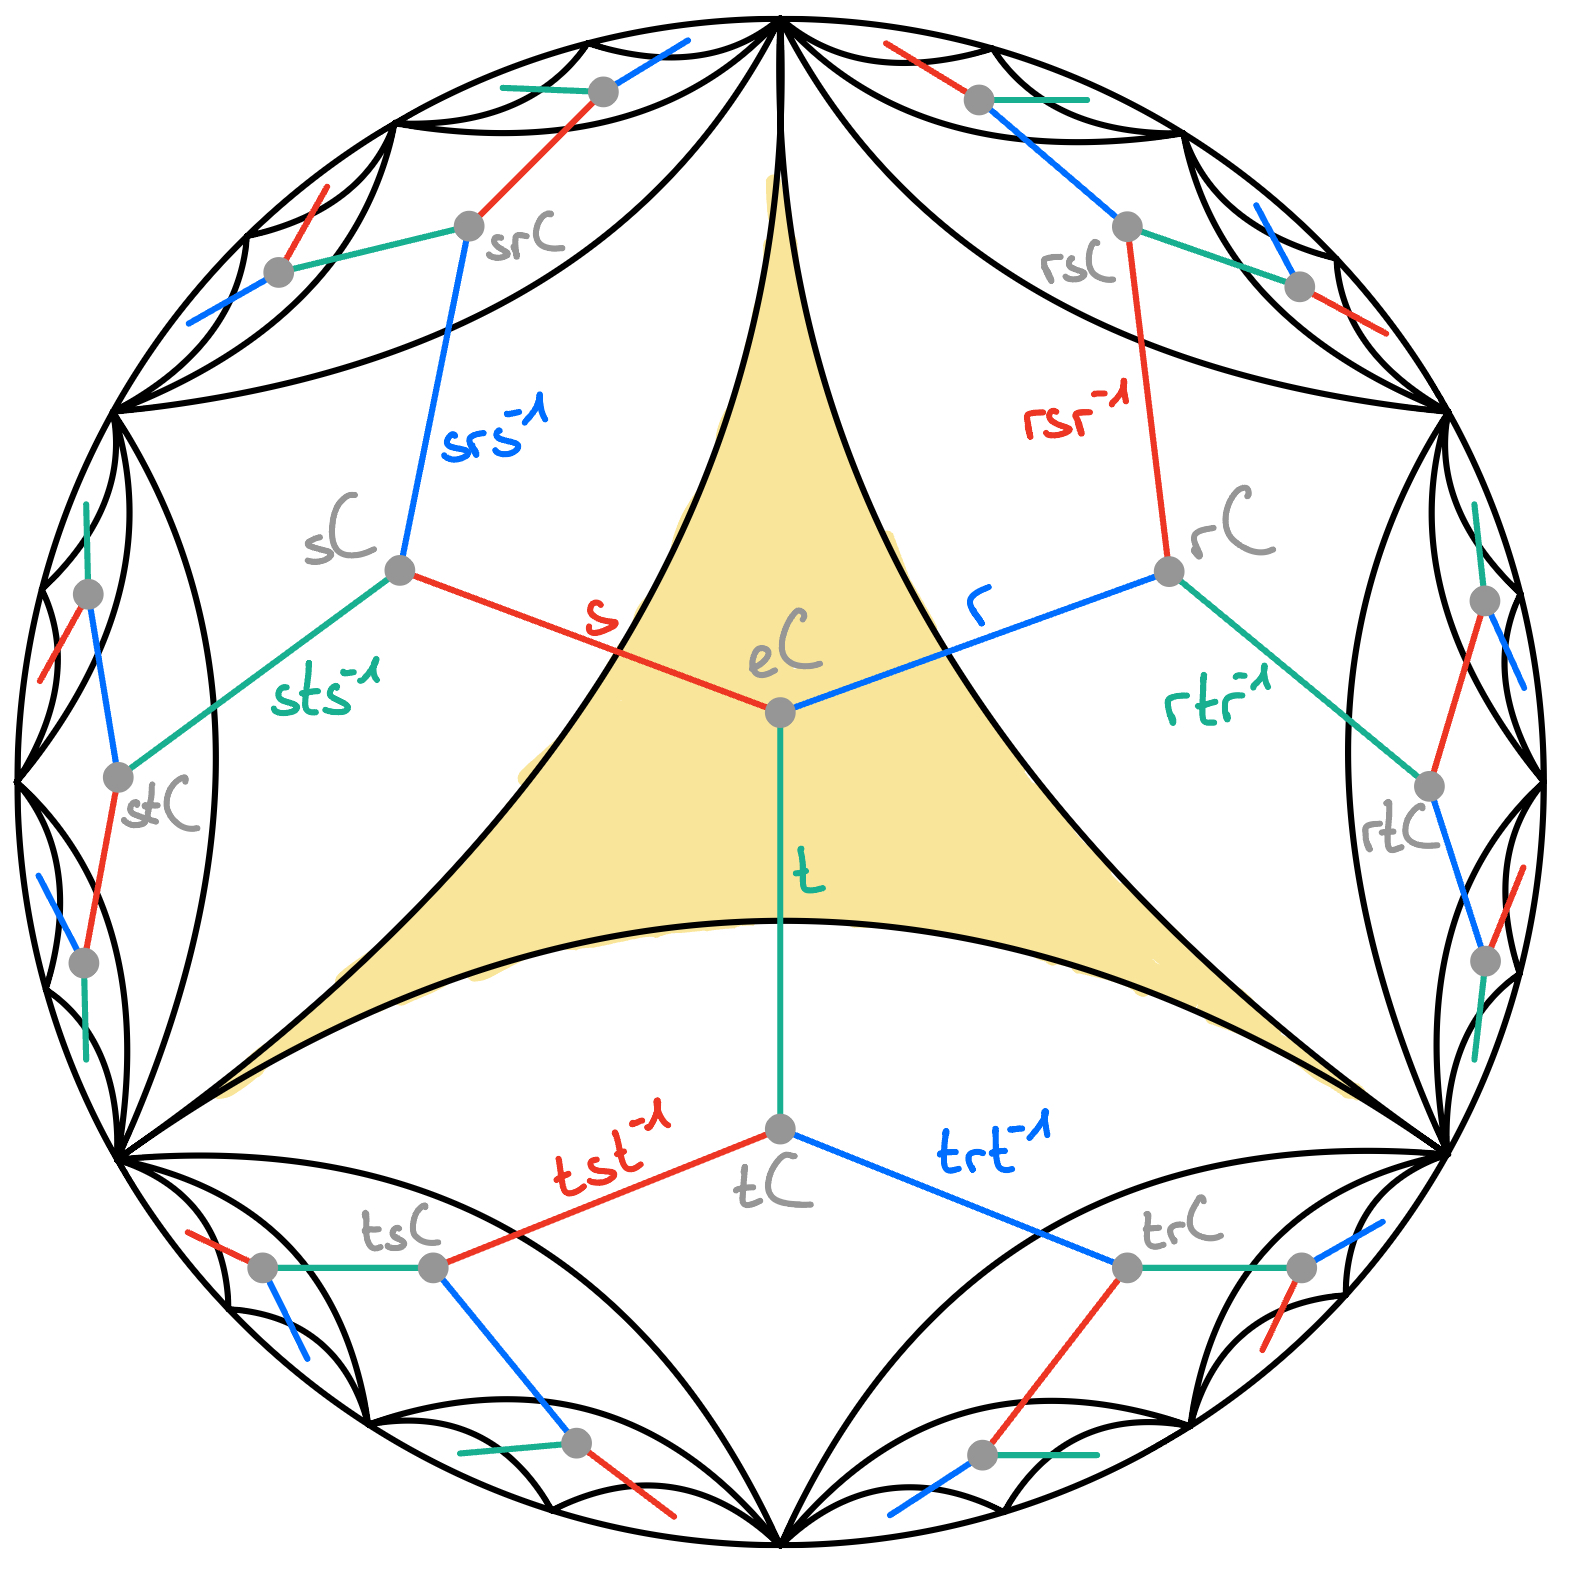
\includegraphics[width=.7\textwidth]{gfx/Chamber graph.png}
        \caption{The chamber graph of \(\faktor{\Z}{2\Z} \ast \faktor{\Z}{2\Z} \ast \faktor{\Z}{2\Z}\).}
    \end{figure}
\end{example}


\newpage
% ***********************************************
\section{The cofinal manifold sequence}
% ***********************************************

We finally have developed enough tools, to construct the desired sequence of subgroups in \(W'\).
Following \Cref{thm:cofinal}, we fix a cofinal doubling sequence \(P_k\), starting in the fundamental chamber \(P_0 = C\) corresponding to the dual representation of \(W\), i.e. we fix a cofinal sequence of two-fold orbifold covers \(C \leftarrow P_1 \leftarrow P_2 \leftarrow \cdots\).
Then, we define the groups \(W_i := \pi_1^{\text{orb}}(P_i) \cap W'\) for \(i \in \{0\} \cup \N\), each inducing a manifold via the quotient \(\faktor{int(WC)}{W_i}\).
Clearly, each \(W_i\) is a subgroup of \(W'\) as well as it is a subgroup of the orbifold fundamental group of the polytope (with orbifold structure) \(P_i\).
Using the theory of orbifold coverings, we observe that the construction of these manifolds implies that they are coverings of the polytopes \(P_i\) for each \(i\).
By \Cref{rmk:groupseries}, the cofinal two-fold tower induces a descending series of fundamental groups of the polytopes \(P_i\).
Intersecting them with the finite index subgroup \(W'\) does not affect the cofinality and thus, the sequence of subgroups formed by the groups \(W_i\) is again cofinal.

\noindent
% To keep track of our progress, we note that to show that \(W'\) is RFRS, it remains to show the following two conditions:
We observe that to show that \(W'\) is RFRS, it remains to show the following two conditions:
\begin{enumerate}
    \item each \(W_i := \pi_1^{\text{orb}}(P_i) \cap W'\) has finite index in the group \(W'\) and
    \item \((W_i)_r^{(1)} = \ker\{W_i \to \Q \otimes_\Z (W_i)_{\text{ab}}\}\) is a subgroup of \(W_{i+1}\).
\end{enumerate}
The first condition is essentially a consequence of the fact that the sequence of orbifold fundamental groups has index precisely two in each step.
To conclude, we prove the following lemma.

\begin{lemma}\label{lem:index}
    % The map \(\phi : \faktor{W_i}{W_{i+1}} \to \faktor{\pi_1^{\text{orb}}(P_i)}{\pi_1^{\text{orb}}(P_{i+1})}, \; g \cdot W_{i+1} \mapsto g \cdot \pi_1^{\text{orb}}(P_{i+1})\) is injective.
    The homomorphism \(\phi : \faktor{W_i}{W_{i+1}} \to \faktor{\pi_1^{\text{orb}}(P_i)}{\pi_1^{\text{orb}}(P_{i+1})}\) is injective.
\end{lemma}
\begin{proof}
    Suppose, \(g,h \in \faktor{W_i}{W_{i+1}}\) with \(\phi(g) = \phi(h)\), which is equivalent to
    % \[g \cdot \pi_1^{\text{orb}}(P_{i+1}) = h \cdot \pi_1^{\text{orb}}(P_{i+1}) \iff g^{-1}h \in \pi_1^{\text{orb}}(P_{i+1}).\]
    \[g \cdot \pi_1^{\text{orb}}(P_{i+1}) = h \cdot \pi_1^{\text{orb}}(P_{k+1}).\] %\iff g \cdot W_{i+1} = h \cdot W_{i+1}\]
    % But \(g, h \in \faktor{W_i}{W_{i+1}}\) and \(W_i = \pi_1^{\text{orb}}(P_{i+1}) \cap W'\) imply \(g^{-1}h = 1_A\) and thus, \(g = h \in A\).
    % But the fact that \(g\) and \(h\) lie in \(\faktor{W_i}{W_{i+1}}\), and the definition of the groups \(W_i\) imply that \(g^{-1}h = 1\) in the quotient \(\faktor{W_i}{W_{i+1}}\).
    Since \(g\) and \(h\) lie in \(\faktor{W_i}{W_{i+1}}\), we have that \(gW_{i+1} = hW_{i+1}\), equivalently \(g^{-1}h \in W_{i+1}\) from what we conclude that \(g = h\) in the quotient \(\faktor{W_i}{W_{i+1}}\) and the result follows. 
\end{proof}

An immediate consequence of this is the following result, we record here.

\begin{corollary}\label{cor:index}
    The index of \(W_{i+1}\) in \(W_i\) is less than or equal to \(2\).
\end{corollary}

% With this insight in hand, we are now able to conclude that the first of the remaining conditions is satisfied by the constructed series of groups.
Based on this observation, we can conclude that the first of the above conditions holds for the constructed sequence of groups.
We state this here as a corollary.

\begin{corollary}
    The index of \(W_i\) in \(W'\) is finite.
\end{corollary}
\begin{proof}
    By the above corollary, we have that the index of \(W_{i+1}\) in \(W_i\) is less than or equal to \(2\).
    % As elaborated on in the beginning of this section, the \(W_i\) form a cofinal descending series of groups.
    % This allows us to conclude that for some \(n \in \N\), we have that \(W_j = \{1\}\) for all \(j \geq n\).
    Thus, for the index of \(W_i\) in \(W'\) we have the upper bound \([W':W_i] \leq 2^i < \infty\) for \(i \in \N\).
\end{proof}

% Verifying the first condition was relatively straightforward.
% However, the final one requires slightly more work.
% We will address it in the last section.


% ***********************************************
\section{Loops bouncing off faces}
% ***********************************************

As discussed in the previous section, we need to show that the rational derived group \((W_i)_r^{(1)}\) is a subgroup of \(W_{i+1}\).
First, recall the following result, addressing abelian quotients.

\begin{lemma}\label{lem:abelianquotient}
    Let \(G\) be a group with normal subgroup \(N \triangleleft G\).
    The quotient group \(\faktor{G}{N}\) is abelian if and only if the derived subgroup \(G^{(1)} = [G, G]\) of \(G\) is contained in the normal subgroup \(N\).
\end{lemma}
\begin{proof}
    \begin{itemize}
        \item[`\(\Rightarrow\)'] As \(N\) is normal in \(G\) and the quotient is abelian, for any \(g,h \in G\) we have that
            \[ghN = gN \cdot hN = hN \cdot gN = hgN \iff g^{-1}h^{-1}gh \in N.\]
            This is equivalent to the commutator \([g, h]\) being in \(N\) for all \(g,h \in G\), therefore \([G, G] \subset N\).
        
        \item[`\(\Leftarrow\)'] As now, \([G, G] \subset N\) for any \(g \in G\) and \(n \in N\), we have
            \[gng^{-1} = gng^{-1}n^{-1}n = [g, n]n.\]
            Since \([G, G] \subset N\), this element is again in \(N\) so that \(N\) is normal in \(G\).
            To see that the quotient by \(N\) is abelian, we take \(g, h \in \faktor{G}{N}\) and calculate
            \[gN \cdot hN = ghN = hgg^{-1}h^{-1}ghN = hg[g^{-1}, h^{-1}]N = hgN = hN \cdot gN.\]
            The result follows directly.
    \end{itemize}\vspace*{-2\parskip}
\end{proof}

\begin{lemma}\label{lem:indextwo}
    Let \(G\) be a group and \(N \leq G\) a subgroup of index two.
    Then, \(N\) is normal in \(G\).
\end{lemma}
\begin{proof}
    Let \(g\) be an element in \(G\).
    As \(N\) has index two in \(G\), we have that either \(g \in N\) or \(g \in G\backslash N\).
    The first case is trivial, as \(gN = N = Ng\) and in the second case we have that \(gN = G \backslash N = Ng\), since cosets partition the group \(G\).
    This implies that \(N\) is normal in \(G\).
\end{proof}

Using these two auxiliary lemmas, we can prove the following intermediate result.

\begin{proposition}\label{prop:factorization}
    The quotient group \(\faktor{W_{i}}{W_{i+1}}\) is either isomorphic to \(\faktor{\Z}{2\Z}\) or the trivial group.
    Furthermore, the quotient map \(W_i \to \faktor{W_i}{W_{i+1}}\) factors through the abelianization and the derived subgroup \((W_i)^{(1)}\) of \(W_i\) is a subgroup of \(W_{i+1}\).
\end{proposition}
\begin{proof}
    The first part is a direct consequence of \Cref{cor:index} and \Cref{lem:indextwo}.
    Thus, the quotient \(\faktor{W_i}{W_{i+1}}\) is in particular abelian and we are able to apply \Cref{lem:abelianquotient}.
    This implies that the derived subgroup \((W_i)^{(1)} = [W_i, W_i]\) is a subgroup of \(W_{i+1}\).
    Stated differently, we have a factorization of \(W_i \to \faktor{W_i}{W_{i+1}}\) through the abelianization \((W_i)_{\text{ab}}\).
\end{proof}
\newpage

\begin{remark}\label{rmk:factorization}
    Recall that by \Cref{rmk:tensoring} torsion elements will not survive in the rational derived subgroup \((W_i)_r^{(1)}\) of \(W_i\), and by \Cref{prop:factorization} we already have that \((W_i)^{(1)}\) is a subgroup of \(W_{i+1}\).
    We claim that it suffices to show that every element \(w \in W_i\) with non-trivial image in the quotient group \(\faktor{W_i}{W_{i+1}}\) is not torsion in the abelianization \((W_i)_{\text{ab}}\).
    This is justified, as by \Cref{prop:factorization}, we have a factorization through the abelianization of \(W_i\).
    Then, since \(w\) is not torsion in \((W_i)_{\text{ab}}\), it will admit a factorization through the torsion-free abelianization.
    \begin{figure}[h!]
        \centering
        \begin{tikzcd}
            W_i \arrow[rr] \arrow[dr] & {} & \faktor{W_i}{W_{i+1}} \cong \faktor{\Z}{2\Z} \\
            {} & \faktor{(W_i)_{\text{ab}}}{\text{Torsion}} \arrow[ru, dashed]
        \end{tikzcd}
    \end{figure}\vspace*{-1\parskip}
    
    \noindent
    In particular, the group \(\faktor{W_i}{W_{i+1}}\) then is a quotient of the torsion-free abelianization \(\faktor{(W_i)_{\text{ab}}}{\text{Torsion}}\).
\end{remark}

In the following we will denote the manifolds \(\faktor{int(WC)}{W_i}\) by \(M_i\) for \(i \in \{0\} \cup \N\) and the projections to the orbifolds \(P_i\) by \(p_i : M_i \to P_i\).
Furthermore, we fix an element \(w\) that is contained in \(W_i\) but not in \(W_{i+1}\), together with a loop \(\gamma\), which represents the element \(w\) in the manifold \(M_i\).

\begin{lemma}\label{lem:loopintersection}
    The loop \(\gamma\) intersects the preimage \(p_i^{-1}(F_i)\) of the face \(F_i\), in which \(P_i\) is doubled to obtain the polytope \(P_{i+1}\), an odd number of times.
\end{lemma}
\begin{proof}
    Project \(\gamma\) down to the polytope \(P_i\) generically, using the projection \(p_i\).
    As the polytopes \(P_i\) have cyclic local group of order two everywhere on their codimension-one faces, the projection of \(\gamma\) gets reflected in the faces of the polytopes \(P_i\).
    Now, consider the face \(F_i\) in which \(P_i\) gets doubled.
    Then, \(p_i(\gamma)\) hits this face an odd number of times, else \(p_i(\gamma)\) would lift to a loop in the double \(P_{i+1}\), and therefore, the element \(w\) represented by \(\gamma\) would lift to the group \(W_{i+1}\).
    This contradicts our choice of \(w\), not being contained in \(W_{i+1}\).
    In particular, observing the loop \(\gamma\) directly up in the manifold \(M_i\), we see it intersecting the preimage \(p_i^{-1}(F_i)\) of the face \(F_i\) an odd number of times, which proves the lemma.
\end{proof}

% To see what is going on, we project \(\gamma\) down to the polytope \(P_i\) generically, using the covering map \(p_i : M_i \to P_i\). %from \(M_i\) to \(P_i\).
% As the polytope \(P_i\) has cyclic local group of order two everywhere on its codimension-\(1\) faces, what we see is a ray bouncing around the orbifold.
% One could think of a polytope with mirrors as its faces and we are watching a ray of light getting reflected in the mirrors.
% Consider the face \(F_i\), in which \(P_i\) is doubled to produce \(P_{i+1}\).
% By our choice of the element \(w\), what we are seeing is that the projection \(p_i(\gamma)\) hits this face \(F_i\) an odd number of times.
% If it would hit \(F_i\) an even number of times, \(p_i(\gamma)\) would lift to a loop in \(P_{i+1}\) and therefore \(w\) would lift to the group \(W_{i+1}\), a contradiction.
% In particular, observing the loop \(\gamma\) up in the manifold \(M_i\), we see \(\gamma\) intersecting the preimage of \(F_i\) in \(M_i\) an odd number of times. % as well.

One might think of the orbifolds \(P_i\) as polytopes that are formed by mirrors, and the loop \(\gamma\) as a closed path formed by a ray of light, being reflected in these mirrors.
This interpretation also motivated the name of this section.
Before proceeding, we want to provide a more explicit picture of the above argument.
We record this in the following remark.

\begin{remark}
    We want to explain what is happening here in a more explicit way.
    To do so, we look at the following picture, which one should think of in a schematic way.
    We see a loop \(\gamma\) (which, strictly speaking, is the projection of a loop in the manifold \(M_i\)) in the polytope \(P_i\), being reflected in the codimension-one faces of \(P_i\).
    The face of interest \(F_i\) is colored in blue and we assume \(\gamma\) to be the orange path, walked around exactly once, starting in the basepoint \(x_0\).
    \begin{figure}[ht!]
        \label{fig:ray}
        \centering
        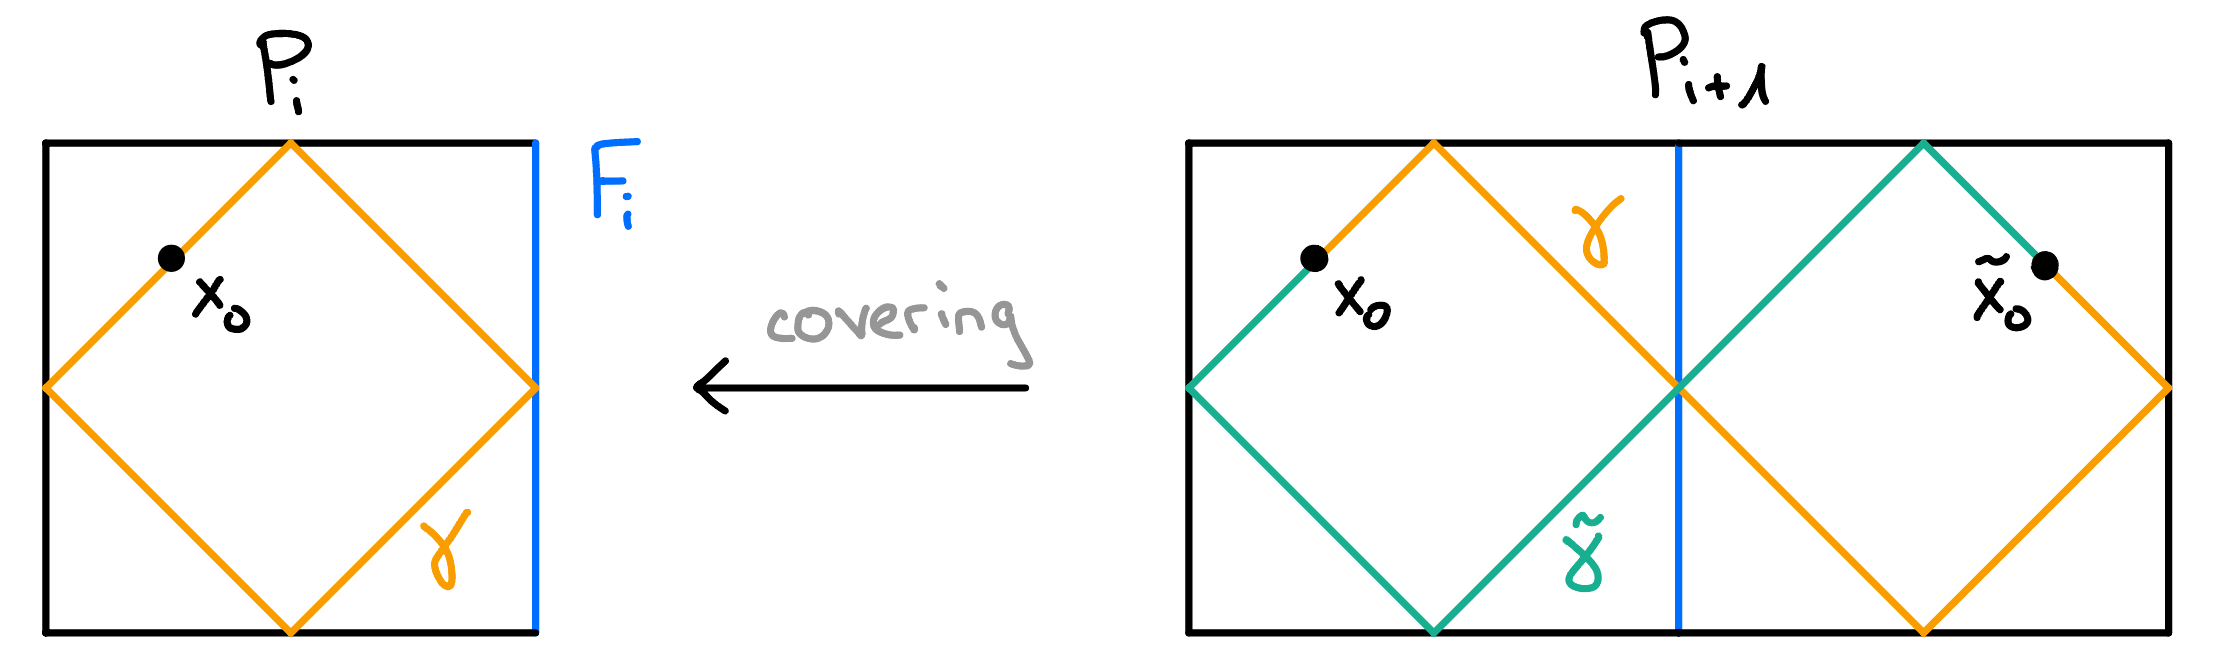
\includegraphics[width=.8\textwidth]{gfx/Ray bouncing in P.png}
    \end{figure}\vspace*{-\parskip}\newpage

    \noindent
    By doubling the polytope \(P_i\) along the face \(F_i\), we land on the right side of this picture.
    Observe that the basepoint \(x_0\) now has a corresponding double, denoted by \(\widetilde{x}_0\).
    The more interesting part is, that now the loop \(\gamma\) gets unwound to a path going from \(x_0\) to \(\widetilde{x}_0\).
    If, on the other hand, we consider the loop \(\gamma^2\), i.e. the loop \(\gamma\) gets run through twice, consequently hitting the face \(F_i\) twice, by our reasoning above, we should see a loop coming from \(\gamma^2\) in the two-fold cover \(P_{i+1}\).
    Indeed, the loop \(\gamma^2\) lifts to a loop \(P_{i+1}\) and is pictured by the concatenated loop \(\widetilde{\gamma} \cdot \gamma\) in \(P_{i+1}\) on the right.
\end{remark}

Now that we have a more intuitive view on our reasoning, we have to deal with one more minor issue.
We will mention it in the following remark, but will omit the details.

\begin{remark}
    Note that we could also have a loop \(\gamma\) like in the left of the following image.
    \begin{figure}[h!]
        \label{fig:badray}
        \centering
        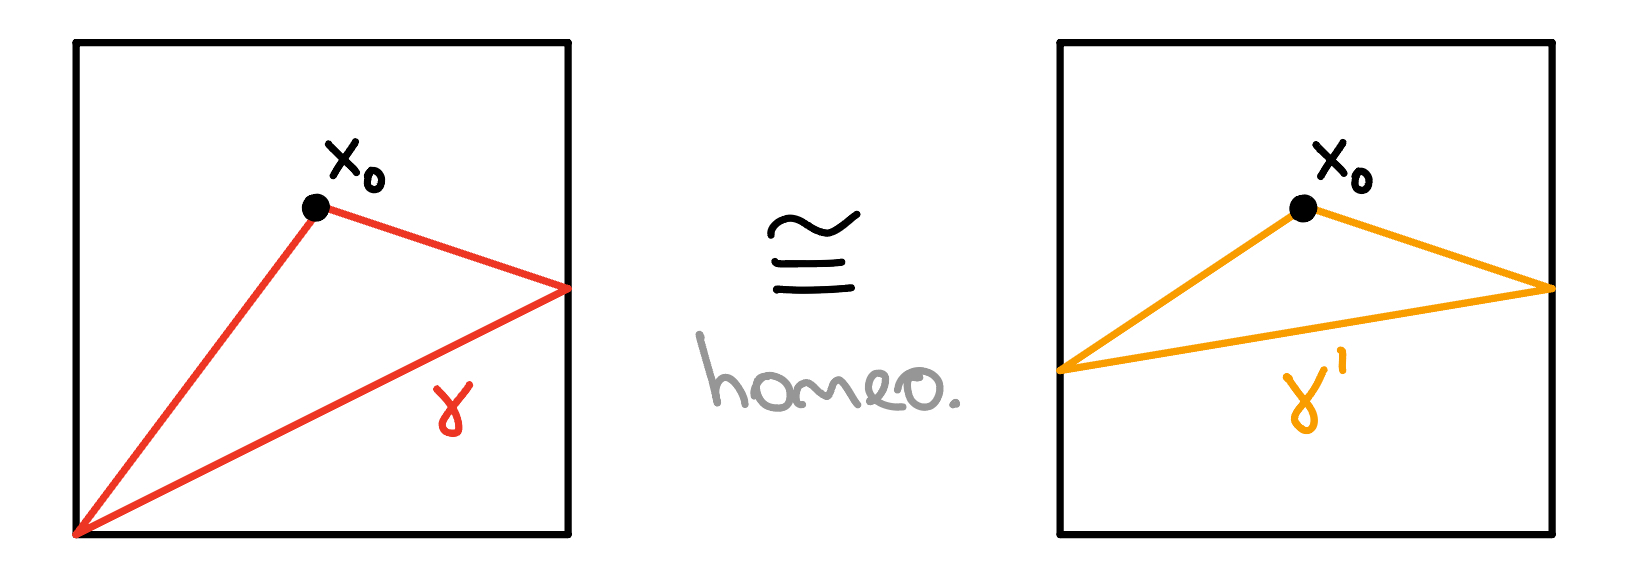
\includegraphics[height=3.2cm]{gfx/Equivalent loops.png}
    \end{figure}\vspace*{-\parskip}

    \noindent
    The difficulty with such loops is that the codimension-\(2\) faces of a polytope also consist of singular points.
    Their local group may very well be different from the local groups of the points in codimension-\(1\) faces.
    Nevertheless, we fortunately do not have to deal with them.
    In fact, we can always find a loop \(\gamma'\), homotopy equivalent to \(\gamma\) and that is only hitting codimension-\(1\) faces.
\end{remark}

In the following, our goal will be to obtain a homomorphism of fundamental groups, from the fundamental group of the manifold \(\pi_1(M_i)\) to the fundamental group of the circle \(\pi_1(S^1)\).
This morphism will be induced by a continuous quotient map.
To make this precise, we have to introduce one more concept, we have not yet mentioned.
This is the fact that the preimage of a face \(F_i\) in the manifold \(M_i\) is two-sided (moreover it is oriented and embedded).
This is a technical condition on the preimage \(p_i^{-1}(F_i) \subset M_i\).
As it will play an important role in the following, we give the definition of what it means to be two-sided.

\begin{definition}
    Let \(M\) be a manifold.
    A submanifold \(F \subset M\) is called \emph{two-sided} in \(M\), if it locally looks like the product with an interval.
    More precisely, there is a neighborhood \(N_F\) with \(N_F \cong F \times (-\varepsilon, \varepsilon)\) for suitable \(\varepsilon > 0\), where the submanifold \(F\) is identified with the fiber \(F \times \{0\}\).
\end{definition}

\noindent
Denote by \(N_{F_i} \subset M_i\) the neighborhood coming from the two-sidedness of the preimage \(p_i^{-1}(F_i) \subset M_i\).
Using this neighborhood, we can construct the morphism in the next lemma.

\begin{lemma}\label{lem:morphism}
    There exists a continuous quotient map \(q : M_i \to S^1\) that induces a homomorphism of groups \(q_* : \pi_1(M_i) \to \pi_1(S^1)\), between the fundamental groups.
\end{lemma}
\begin{proof}
    We will give an constructive proof.
    To do so, introduce an equivalence relation on the points in the manifold \(M_i\) as follows:
    \[x \sim y \qquad :\iff \qquad x,y \in M_i \backslash N_{F_i} \quad\text{or}\quad x = y.\]
    Equip the quotient \(\faktor{M_i}{\sim}\) with the quotient topology.
    Then, by passing to this quotient, we see a double cone with identified cone points.
    \begin{figure}[h!]
        \label{fig:doublecone}
        \centering
        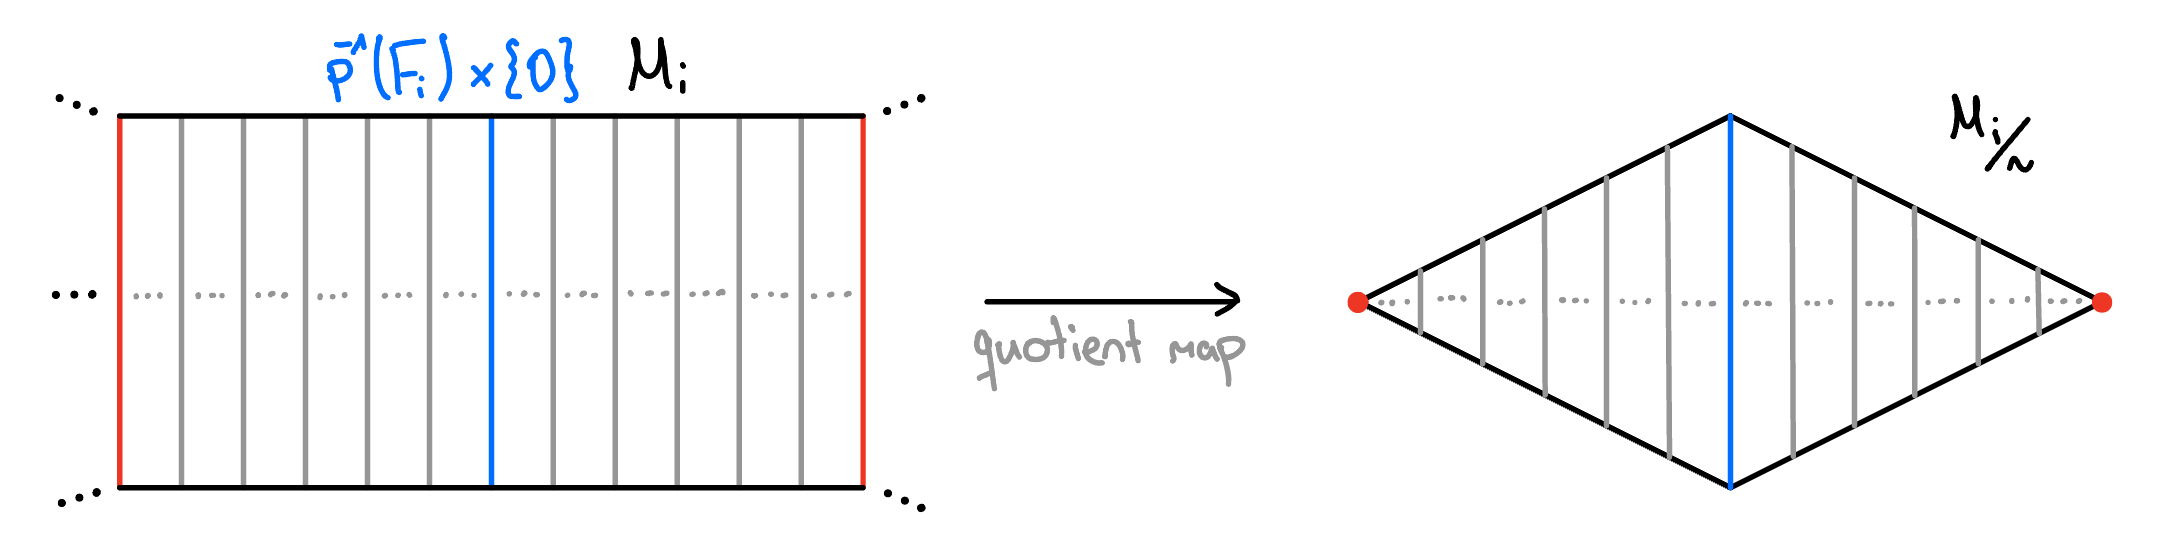
\includegraphics[width=.7\textwidth]{gfx/Quotient 1.png}
    \end{figure}\vspace*{-\parskip}
    
    \noindent
    Continuing from this space on, we have to pass to another quotient.
    Namely, we have to collapse each of the fibers \(p_i^{-1}(F_i) \times \{z\}\) for every \(z \in (-\varepsilon, \varepsilon)\) to a single point.
    This can be done by introducing another equivalence relation on the quotient space \(\faktor{M_i}{\sim}\;\) by 
    \[x \sim_1 y \qquad :\iff \qquad \exists\; z \in (-\varepsilon, \varepsilon): \; x,y \in p_i^{-1}(F_i) \times \{z\}.\]
    Equip this quotient again with the quotient topology and by passing to this further quotient, we are left with the interval \((-\varepsilon, \varepsilon)\), whose endpoints are identified.
    \begin{figure}[ht!]
        \label{fig:circle}
        \centering
        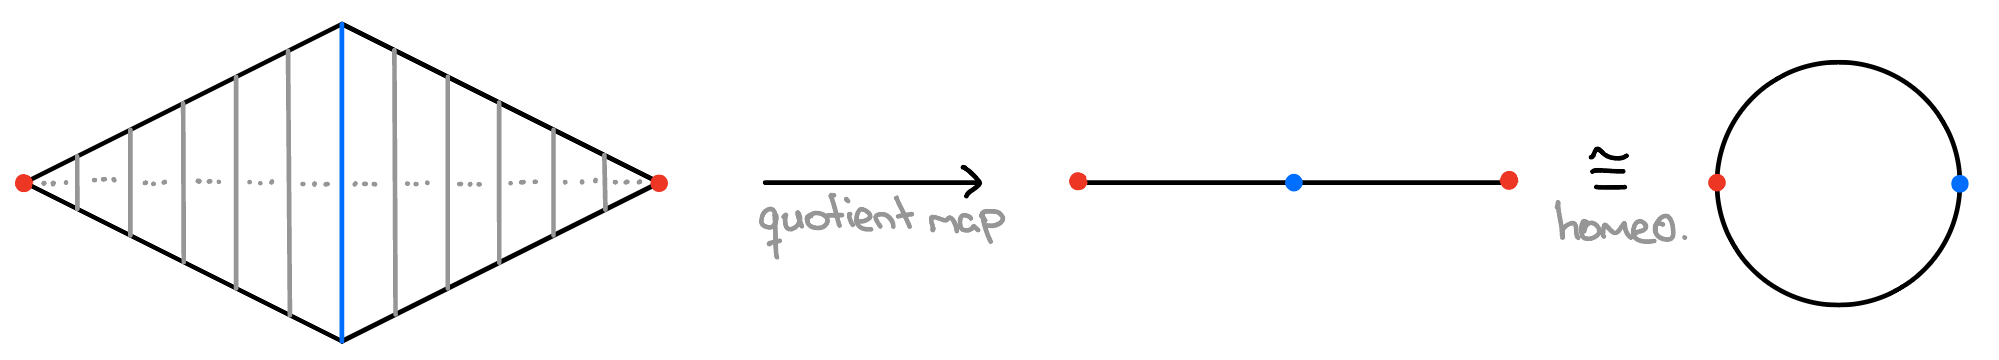
\includegraphics[width=.7\textwidth]{gfx/Quotient 2.png}
    \end{figure}\vspace*{-\parskip}

    \noindent
    As all the quotient spaces carry the quotient topology that is defined just right to make such constructions work, we only have to think about the red point.
    Consider the composed quotient map \(q : M_i \to S^1\) and a neighborhood \(U\) around the red point.
    Then, \(U\) is of the form \([-\varepsilon, -\varepsilon + \delta) \cup (\varepsilon - \delta, \varepsilon]\) for some \(\delta \in (0, \varepsilon)\) and it is open in the quotient if and only if its preimage \(p_i^{-1}(U)\) is open in \(M_i\).
    The preimage of \(U\) in \(M_i\) is of the form
    \[q^{-1}(U) = M_i \backslash N_{F_i} \cup p_i^{-1}(F_i) \times [-\varepsilon, -\varepsilon + \delta) \cup p_i^{-1}(F_i) \times (\varepsilon - \delta, \varepsilon],\]
    which is open, as its complement \(M_i \backslash q^{-1}(U) = p_i^{-1}(F_i) \times [-\varepsilon + \delta, \varepsilon - \delta]\) is closed in \(M_i\).
    \begin{figure}[h!]
        \label{img:quotientnbhd}
        \centering
        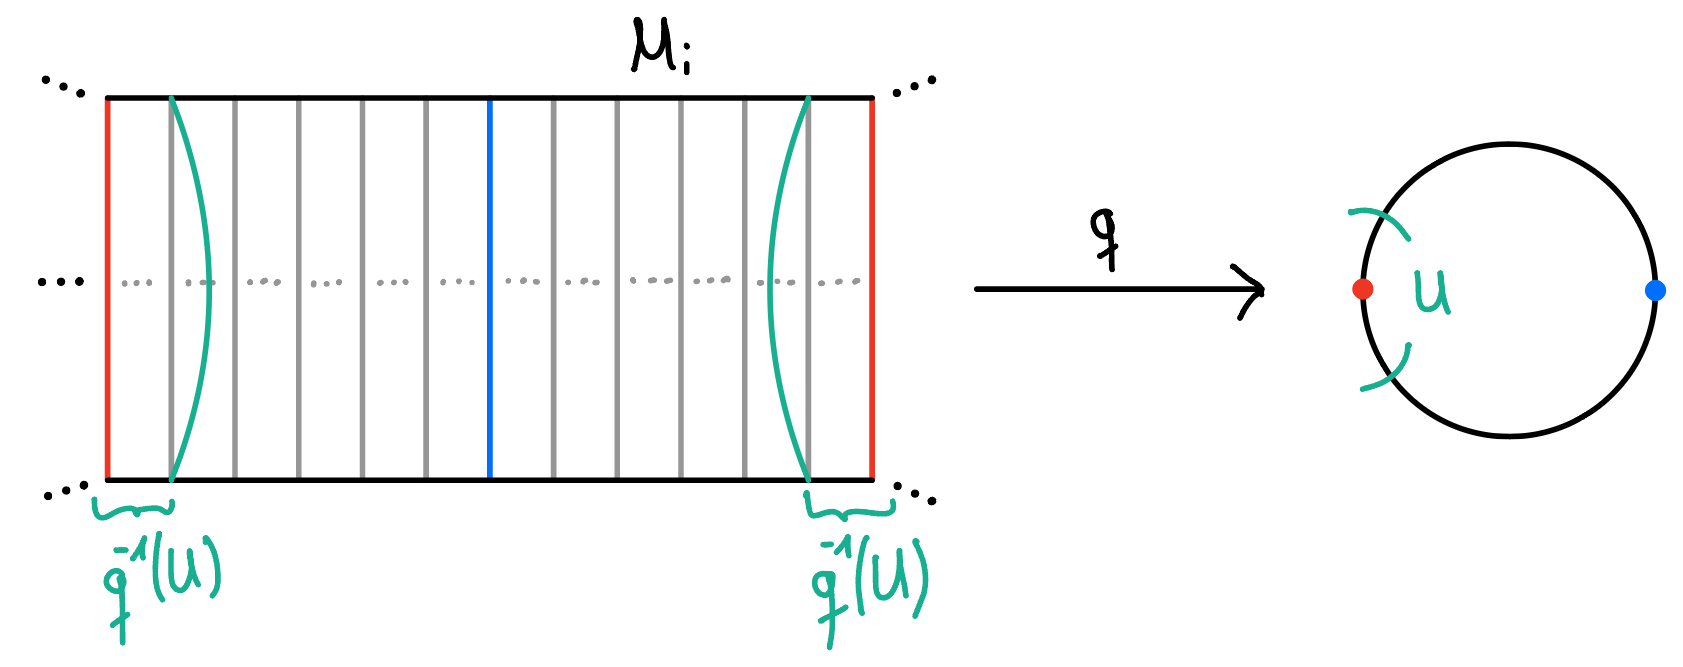
\includegraphics[width=.5\textwidth]{gfx/Quotient neighborhood .png}
    \end{figure}\vspace*{-2\parskip}

    \noindent
    Thus, the quotient map \(q : M_i \to S^1\) is continuous and therefore, it induces the desired homomorphism \(q_* : \pi_1(M_i) \to \pi_1(S^1)\) between the corresponding fundamental groups.
\end{proof}

We will now use the developed results to prove the following key-lemma.
But before we do so, we want to add one more remark.

\begin{remark} % TODO: fulfill this remark
    % We want to elaborate on the term `projecting generically' we used in the proof of \Cref{lem:loopintersection} now in the context of the two-sidedness of \(p_i^{-1}(F_i)\) in the manifold \(M_i\).
    % The additional adjective `generically' means that the composition
    Note that in the proof of \Cref{lem:loopintersection}, we used the term `projecting generically'.
    We implicitly already used there that the preimage \(p_i^{-1}(F_i)\) is two-sided.
    The addendum `generically' means that \(p_i : M_i \to P_i\) composed with the projection \(P_i \to (-\varepsilon, \varepsilon)\), to the interval coming from the neighborhood \(p_i^{-1}(N_{F_i})\) in \(M_i\), is actually injective in every neighborhood of an intersection of \(\gamma\) and \(F_i\).
\end{remark}

\begin{lemma}\label{lem:infiniteorder}
    The loop \(\gamma\) represents an element of infinite order in the abelianization \((W_i)_{\text{ab}}\).
\end{lemma}
\begin{proof}
    By \Cref{lem:loopintersection}, we know that \(\gamma\) intersects the preimage of \(F_i\) in \(M_i\) an odd number of times.
    Thus, projecting \(\gamma\) down to \(S^1\), using the continuous map \(q\) from \Cref{lem:morphism}, we see that the projection has to wind around the circle an odd number of times.
    For that reason, using the induced morphism \(q_*\), we see that \(\gamma\) has to represent an non-trivial element in \(\pi_1(S^1)\).
    But since \(\pi_1(S^1) \cong \Z\), this immediately implies that \(\gamma\) represents an element of infinite order and moreover, since \(\Z\) is abelian, this implies that \(\gamma\) represents an element of infinite order in \(\pi_1(M_i)_{\text{ab}}\), i.e. \(w\) has infinite order in \(\pi_1(M_i)_{\text{ab}} \cong (W_i)_{\text{ab}}\) as claimed.
\end{proof}

\begin{corollary}\label{cor:looptwo}
    The loop \(2\gamma\) in \(M_i\) represents a non-trivial element in the group \(\Q \otimes_\Z \faktor{W_i}{(W_i)_r^{(1)}}\).
\end{corollary}
\begin{proof}
    By \Cref{lem:infiniteorder}, \(\gamma\) represents an element of infinite order in the abelianization \((W_i)_{\text{ab}}\).
    In particular, this element cannot be contained in the rationally derived subgroup \((W_i)_r^{(1)}\) and the loop \(2\gamma\) has to also represent an element of infinite order with this property.
    This implies that \(2\gamma\) represents an element that survives in the group \(\Q \otimes_\Z \faktor{W_i}{(W_i)_r^{(1)}}\), as claimed.
\end{proof}

\begin{corollary}
    The finite index subgroup \(W'\) of the right-angled Coxeter group \(W\) is RFRS.
\end{corollary}
\begin{proof}
    Since \(\gamma\) is a representative of the element \(w\), we have that \(2\gamma\) is a representative of the element \(w^2\).
    Thus, by \Cref{cor:looptwo} \(w^2\) is not contained in the rational derived subgroup \((W_i)_r^{(1)}\).
    But by \Cref{cor:index}, the index of \(W_{i+1}\) in the group \(W_i\) is less than or equal to two, which implies that \(w^2\) has to be contained in \(W_{i+1}\).
    Considering the factorization from \Cref{rmk:factorization}, we conclude that \(\faktor{W_i}{W_{i+1}} \cong \faktor{\Z}{2\Z}\) is a quotient of the torsion-free abelianization \(\faktor{(W_i)_{\text{ab}}}{\text{Torsion}}\).
    In particular, we have finally established that every element mapping non-trivially to the group \(\faktor{W_i}{W_{i+1}}\) is not torsion in the abelianization \((W_i)_{\text{ab}}\), and by the discussion in \Cref{rmk:factorization}, we can conclude that \((W_i)_r^{(1)}\) is a subgroup of \(W_{i+1}\).
    That was the only part missing for \(W'\) to be RFRS and therefore, we have finally proven the main theorem.
\end{proof}

% To see that the loop \(\gamma\) represents an element of infinite order in \(W_i\), we will construct a morphism of fundamental groups.
% Namely, from the fundamental group \(\pi_1(M_i)\) of the manifold \(M_i\) to the fundamental group of the circle \(\pi_1(S^1)\).
% If \(\gamma\) maps non-trivially to \(\pi_1(S^1)\), it has to represent an element of infinite order, as \(\pi_1(S^1) \cong \Z\).

% The generic projection of \(\gamma\) down to the orbifold \(P_i\) implies that in the projection of the neighborhood \(N_{F_i}\), coming from the two-sidedness, the ray \(\gamma\) is injective, i.e. we don't just walk up to the face and go back without getting reflected.
% As a consequence, in the manifold \(M_i\), the ray \(\gamma\) has to really intersect the preimage of \(F_i\).
% To construct said morphism, we will continue by collapsing all the points not contained in the neighborhood of the preimage of the face \(F_i\).
% This means, we define an equivalence relation on the points in \(M_i\) as follows:
% \begin{equation*}
%     x \sim y  \qquad :\iff \qquad x, y \in M_i \backslash N_{F_i} \quad\text{or}\quad x = y.
% \end{equation*}

% By passing to the quotient \(\faktor{M_i}{\sim}\), we collapse the endpoints of the closure \(\overline{N} \cong F_i \times [-\varepsilon, \varepsilon]\).
% Now, further collapse the single fibers \(F_i \times \{z\}\) for all \(z\) in the open interval \((-\varepsilon, \varepsilon)\).
% What we visually see, already is the one-dimensional sphere \(S^1\).
% We already mentioned that the generic projection implies that \(\gamma\) is injective in this neighborhood \(N\).
% This implies that \(\gamma\) actually intersects the face \(F_i\).

% We now want to describe the space, arising by collapsing the manifold \(M_i\) relative to this equivalence relation, i.e. the quotient space \(\faktor{M_i}{\sim}\).
% As all the points outside the neighborhood \(N_{F_i}\) get identified, we see a double cone with identified cone points.
% \begin{figure}[h!]
%     \label{fig:doublecone}
%     \centering
%     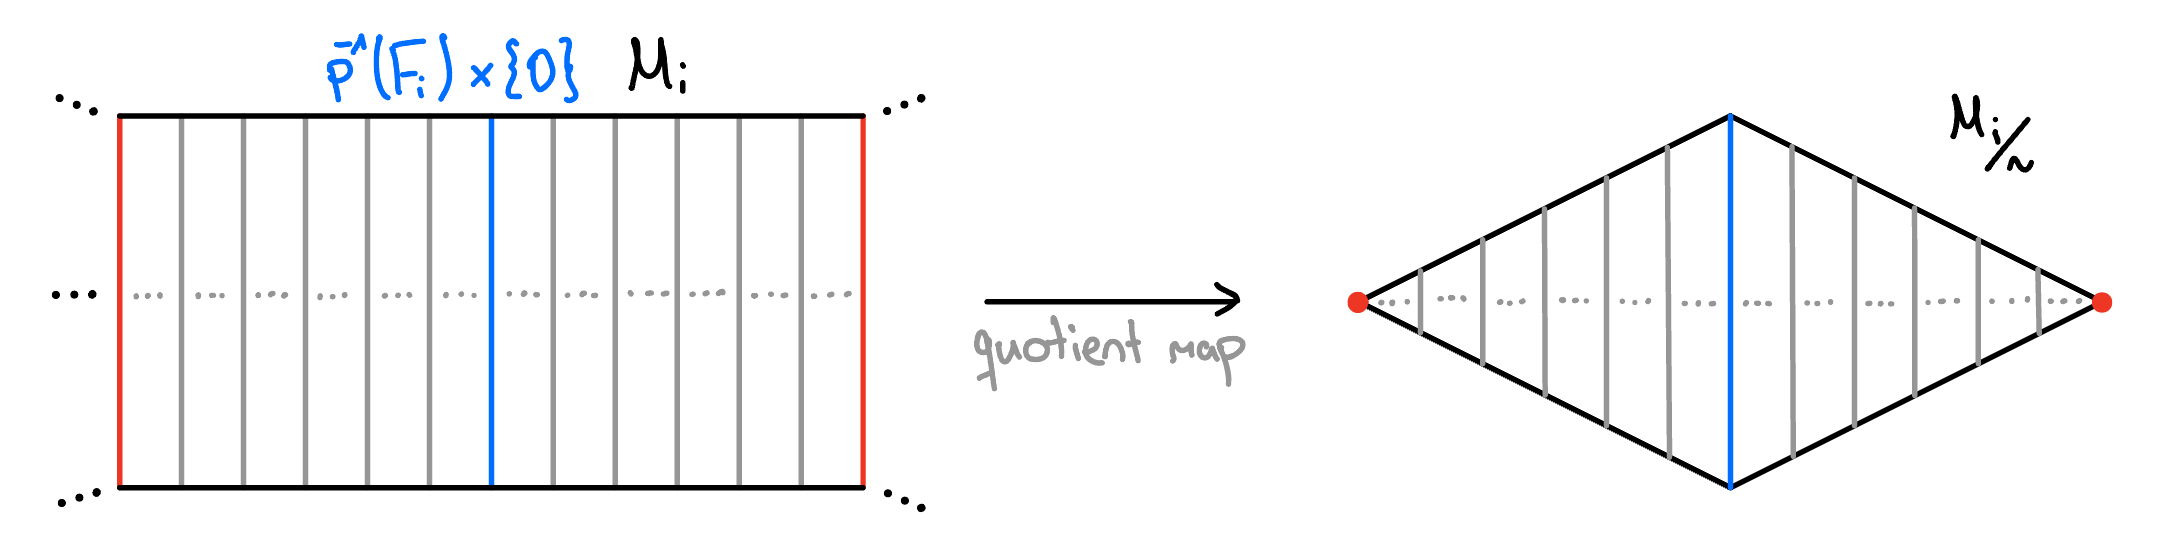
\includegraphics[width=.8\textwidth]{gfx/Quotient 1.png}
% \end{figure}

% This does not yet yield the desired morphism of fundamental groups.
% We have to pass to another quotient by collapsing each of the fibers \(p_i^{-1}(F_i) \times \{z\}\), for every \(z\) in the open interval \((-\varepsilon, \varepsilon)\), to a single point.
% One is then left with the following picture.
% \begin{figure}[ht!]
%     \label{fig:circle}
%     \centering
%     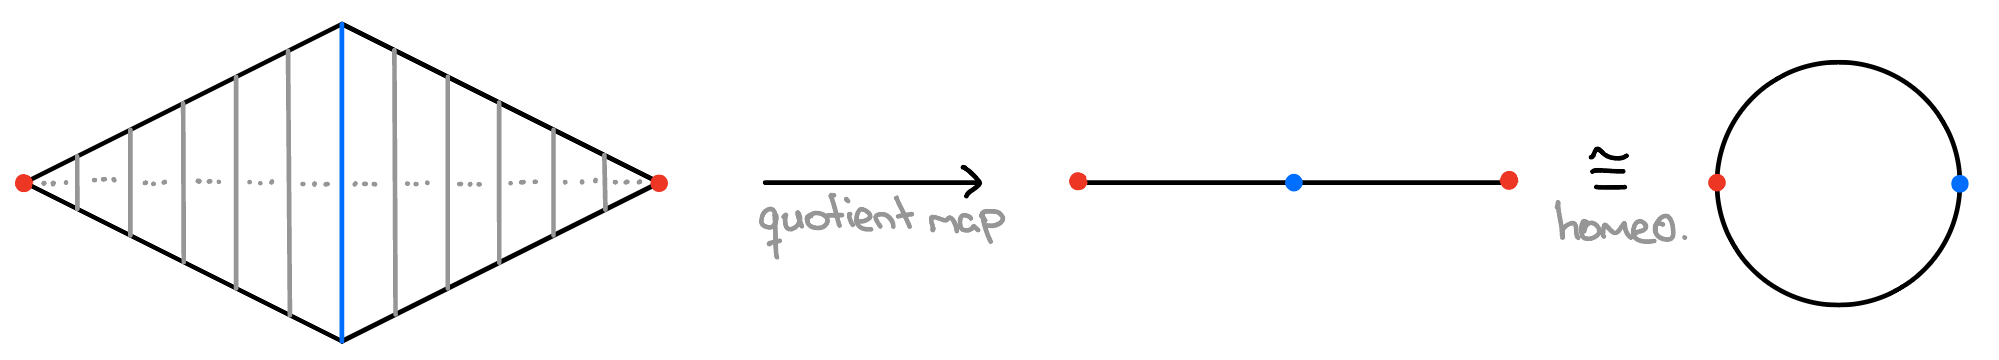
\includegraphics[width=.9\textwidth]{gfx/Quotient 2.png}
% \end{figure}

% The quotient topology is defined just right to make such constructions work.
% Indeed, the only point we have to think about is the red one.
% A neighborhood \(U := (\varepsilon - \delta, \varepsilon] \cup [-\varepsilon, -\varepsilon + \delta)\) for some \(\delta \in (0, \varepsilon)\) around it in the line (or the circle) is open, if and only if its preimage under the composed quotient map is open in the manifold \(M_i\).
% The preimage of \(U\) in the manifold \(M_i\) is the union \(p_i^{-1}(F_i) \times [-\varepsilon, -\varepsilon + \delta) \cup p_i^{-1}(F_i) \times (\varepsilon - \delta, \varepsilon]\) and the complement of the preimage in \(M_i\) is of the form \(p_i^{-1}(F_i) \times [-\varepsilon + \delta, \varepsilon - \delta]\), which is closed.
% \begin{figure}[h!]
%     \label{img:quotientnbhd}
%     \centering
%     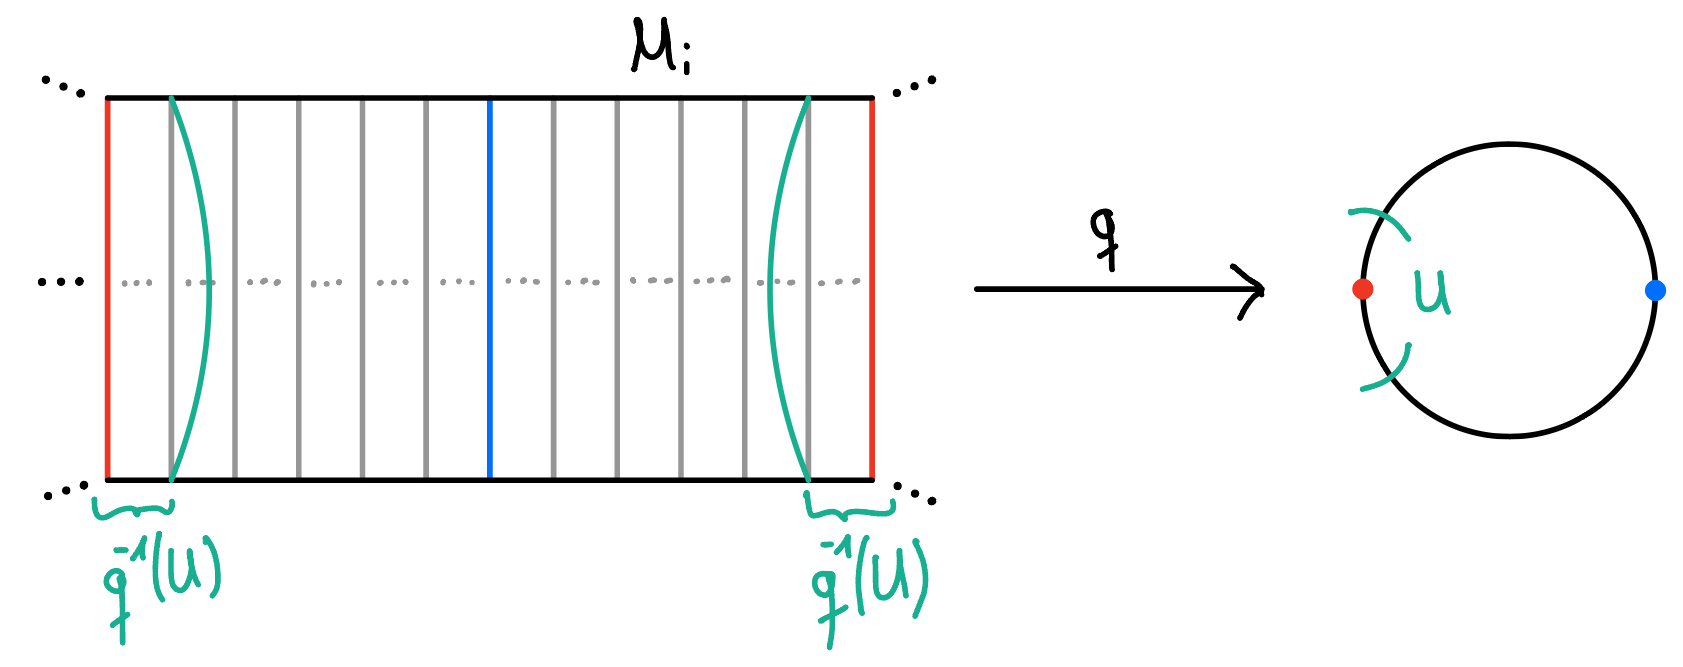
\includegraphics[width=.7\textwidth]{gfx/Quotient neighborhood .png}
% \end{figure}

% \noindent
% Thus, the quotient map to the circle is continuous. % and induces a homomorphism of groups between the fundamental groups \(\pi_1(M_i)\) and \(\pi_1(S^1) \cong \Z\).
% A continuous map between two topological spaces induces a homomorphism between their fundamental groups, so that we get the desired morphism from \(\pi_1(M_i)\) to \(\pi_1(S^1) \cong \Z\), induced by the composed quotient map \(q\).

% Recalling the discussion above, we know that the loop \(\gamma\), intersects the preimage of \(F_i\) an odd number of times in \(M_i\).
% Projecting it down to \(S^1\), we see that the projection has to wind around the circle at least once and for that reason has to represent a non-trivial element in \(\pi_1(S^1)\).
% This implies that the element \(w\), represented by the loop \(\gamma\), has to have infinite order in \((W_i)_\text{ab}\) and therefore is not contained in the rationally derived subgroup \((W_i)_r^{(1)}\). % and therefore is contained in \(\Q \otimes_\Z \faktor{W_i}{(W_i)_r^{(1)}}\).
% Thus, the loop \(2\gamma\) is non-trivial in the group \(\Q \otimes_\Z \faktor{W_i}{(W_i)_r^{(1)}}\). %, from what we deduce that it does not represent any torsion.
% As \(\gamma\) is a representative of \(w\), the loop \(2\gamma\) is a representative of \(w^2\) and it immediately follows that \(w^2 \notin (W_i)_r^{(1)}\), as it cannot be torsion by preceding argument.

% But by the fact that we have \([W_i: W_{i+1}] \leq 2\), the element \(w^2\) has to be contained in \(W_{i+1}\) and we see that the group \(\faktor{W_i}{W_{i+1}} \cong \faktor{\Z}{2\Z}\) is a quotient of the torsion-free abelianization, \(\faktor{(W_i)_{\text{ab}}}{\text{Torsion}} \cong \Q \otimes_\Z (W_i)_{\text{ab}}\) by the before mentioned factorization.
% Thus, we have finally shown that every element mapping non-trivially to the quotient \(\faktor{W_i}{W_{i+1}}\) is not torsion, allowing us to deduce that \((W_i)_r^{(1)}\) is a subgroup of \(W_{i+1}\), which completes the proof.